\documentclass[10pt]{article}
\linespread{0.95}\selectfont
\usepackage[margin=0.82in]{geometry}
\usepackage{graphicx,booktabs,amsmath,hyperref,enumitem}
\hypersetup{colorlinks=true,urlcolor=blue,citecolor=blue,linkcolor=blue,pdftitle={From Verifier-Guided Program Synthesis to Provenance-Aware Test-Time Inference for ARC-AGI},pdfauthor={Yuzhe Ma}}
\title{From Verifier-Guided Program Synthesis to Provenance-Aware Test-Time Inference for ARC-AGI}
\author{Yuzhe Ma\\\small University of Adelaide\\\small \texttt{a1918429@adelaide.edu.au}\\\small \url{https://github.com/jimmy5566/arc-verifier-guided-program-synthesis}}
\date{Research preprint draft --- September 2026}
\begin{document}
\maketitle

\begin{abstract}
ARC-style reasoning tasks require inferring a grid transformation from a few examples while the correct test output is unavailable during inference. This project studies a reliable test-time inference workflow rather than claiming a general ARC solver. The system separates neural candidate generation, typed symbolic representations, deterministic execution, hard train-pair verification, exact-output deduplication with provenance, and fixed target-blind selection. The research trajectory moved from bounded symbolic libraries through Macro DSL failure analysis to a RuleSpec pipeline and public pretrained model candidate search. On one 60-task cohort frozen before inference and target access, a provenance-aware two-attempt method solved 21 tasks versus 18 for a baseline; the paired exact p-value was 0.375, so the observation is directional rather than statistically significant. Across a frozen30 diagnostic, candidate existence (21/30) substantially exceeded likelihood Top-1 success (9/30), motivating a distinction between generation and selection. We also report negative results, train-only representability audits, and a CPU-only replay showing that dynamic four-worker scheduling can reduce modeled makespan without altering inference semantics.
\end{abstract}

\section{Introduction}
ARC was proposed as a setting for studying skill acquisition and abstract reasoning from few examples \cite{chollet2019measure}. ARC-AGI-2 and the ARC Prize provide a related constrained evaluation context \cite{arcprize2026}. In such settings, a single accuracy obscures whether a system failed to represent a rule, generate a candidate, select an existing candidate, or execute robustly. This project therefore asks: \emph{can a verifier-guided pipeline make test-time reasoning more reliable and diagnosable while keeping evaluation target-blind?}

The contribution is primarily experimental and systems-oriented. The author designed the experiments and implemented the symbolic/RuleSpec components, deterministic executor and verifier, augmentation and deduplication pipeline, candidate provenance, ranking diagnostics, frozen-cohort method, and multi-GPU operation. Public Qwen and NVARC-derived assets are external dependencies, not author-trained checkpoints. Results are intentionally scoped: diagnostic, train-only, held-out, and systems measurements are not combined.

\paragraph{Research questions.} \textbf{RQ1:} How should representation capacity, neural candidate generation, and candidate selection be separated and measured? \textbf{RQ2:} Can provenance-aware, target-blind grid-level selection improve two-attempt exact success relative to likelihood-only ranking? \textbf{RQ3:} How can inference be scaled operationally without changing the solver's semantics?

\section{Related work}
ARC foregrounds generalization from sparse examples \cite{chollet2019measure}. ARC-specific work has paired program representations with neural-guided bidirectional search \cite{alford2021neuralguided} and explored inductive logic programming over object-centric DSLs \cite{rocha2024ilp}. More broadly, neural-symbolic research studies learned representations alongside explicit reasoning \cite{garcez2015neurosymbolic}. Candidate-search work considers diverse-path aggregation \cite{wang2023selfconsistency} and deliberate branching \cite{yao2023treeofthoughts}; here the focus is instead a fixed, target-blind grid-level selector with logged provenance.

This work uses public Qwen-family models \cite{qwen3} through the Transformers ecosystem \cite{wolf2020transformers}, but studies their behavior inside a constrained inference architecture rather than training a new foundation model. The grid serialization and selected candidate-search concepts were independently reimplemented after an interface/provenance audit of NVARC \cite{nvarc}; training code, LoRA/TTT implementation, datasets, and submission code were not reused. The current project is not a comparison against these external works.

\section{Problem setting}
Each task provides training input/output grids and a test input. A candidate is acceptable to the symbolic path only if deterministic execution exactly matches every training output. For neural grid candidates, train pairs inform prompts and train-only scores, but not hidden test targets. We distinguish three outcomes: (i) \emph{Any-of-K} candidate recall, scored after freezing, asks whether any candidate equals the target; (ii) Top-1 asks whether the predeclared first ranked output is exact; and (iii) two-attempt exact success asks whether either of two distinct predeclared outputs is exact. Any-of-K is diagnostic, not a deployable accuracy.

\section{Symbolic and neuro-symbolic architecture}
The symbolic path is \emph{evidence extraction $\rightarrow$ rule recognition $\rightarrow$ parameter inference $\rightarrow$ RuleSpec $\rightarrow$ deterministic execution $\rightarrow$ hard verification}. Typed values, selectors, and bindings make intermediate assumptions inspectable. The hard verifier establishes train consistency; it cannot certify that a test output is correct.

Early bounded libraries established an interpretable but weak reference on 1,000 official training tasks. V0 produced 14 standalone exact task solves (and thus 14 cumulative solves). V1 object solvers produced 6 standalone solves, of which 4 were newly added over V0, raising the V0+V1 union to 18. V2 relation/composition solvers also produced 6 standalone solves, but all overlapped the V0+V1 union: they added 0 and left cumulative coverage at 18. A V2 Qwen3-8B Macro DSL pipeline completed both frozen 50-task symbolic and direct-parameter pilot conditions with 0 exact solves. The retained failure analysis attributed the bottleneck to planner/interface and parameter grounding rather than claiming that deterministic verification was defective.

\begin{figure}[t]
\centering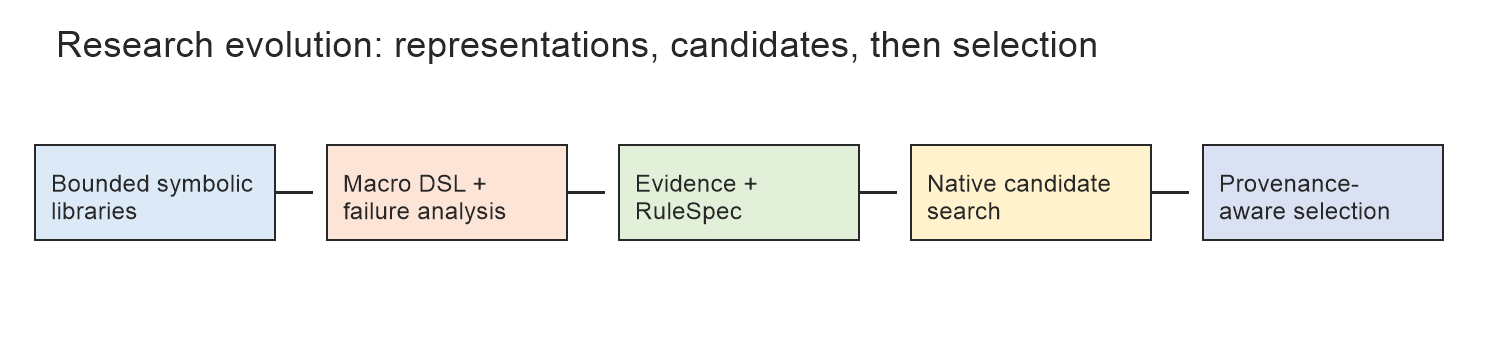
\includegraphics[width=\linewidth]{figures/research_evolution.png}
\caption{Evidence-backed research evolution. The sequence represents changes in scientific focus, not monotonically improving benchmark scores.}
\label{fig:evolution}
\end{figure}

RuleSpec was introduced to make representation capacity separately testable. In a frozen30 train-only construction audit, generic typed semantic extensions increased exact train coverage from 3/30 to 10/30 with no recorded regressions. The audit used train facts and exact hard verification without test-output access. It therefore provides representability evidence, not end-to-end unseen-task accuracy. Remaining failures clustered in repeat motifs, composition/state updates, sequences, progressive spacing, and conditional construction.

\section{Test-time candidate generation}
The native path uses a public ARC-specific Qwen-derived checkpoint with a verified NVARC-compatible grid serialization contract. It applies fixed reversible geometric, color, and order views; generates candidate grids through greedy or bounded branch decoding depending on the frozen experiment; and exactly deduplicates outputs. Deduplication preserves origin support where the artifact format permits it. Candidate scoring uses fixed train-only likelihood-style features, and the second submitted output is the next distinct grid in the same fixed ordering.

This decomposition avoids treating a model score as correctness. In one eight-task untouched multi-view ranker evaluation, every reported ranking method had 3/8 Any-of-K and 2/8 Top-1. A clean five-task TTT validation showed 1/5 to 2/5 candidate recall and 1/5 Top-1 under the fixed TTT pool, but its scale is too small to establish broad benefit. TTT safety checks documented adapter reset, unchanged base-model fingerprints, and memory below a 21 GiB gate; these are operational properties, not solution-quality claims.

\section{Candidate verification and selection}
The central analysis asks what happens after a correct candidate exists. Frozen30 likelihood forensics found correct candidates for 21/30 tasks, but likelihood Top-1 solved only 9/30; the median correct-candidate rank was two. Thus, growing a candidate pool and selecting from it are experimentally distinct problems.

A partial frozen30 A/B/C/D diagnostic separated bounded search from selection. A used the historical pool and likelihood, C added fixed 32-by-4 branch search, and D applied support plus persisted-likelihood selection to C's frozen pool. Only 25 fully checkpointed tasks entered the fixed subset; five incomplete tasks were excluded before scoring. Search increased diagnostic recall from 19/25 to 22/25 (A to C), while Top-1 changed from 9/25 to 8/25. D retained 22/25 recall, restored 9/25 Top-1, and achieved 13/25 two-attempt exact outcomes. This supports a hypothesis of complementary generation and selection mechanisms, not causal generalization beyond that diagnostic subset.

\begin{figure}[t]
\centering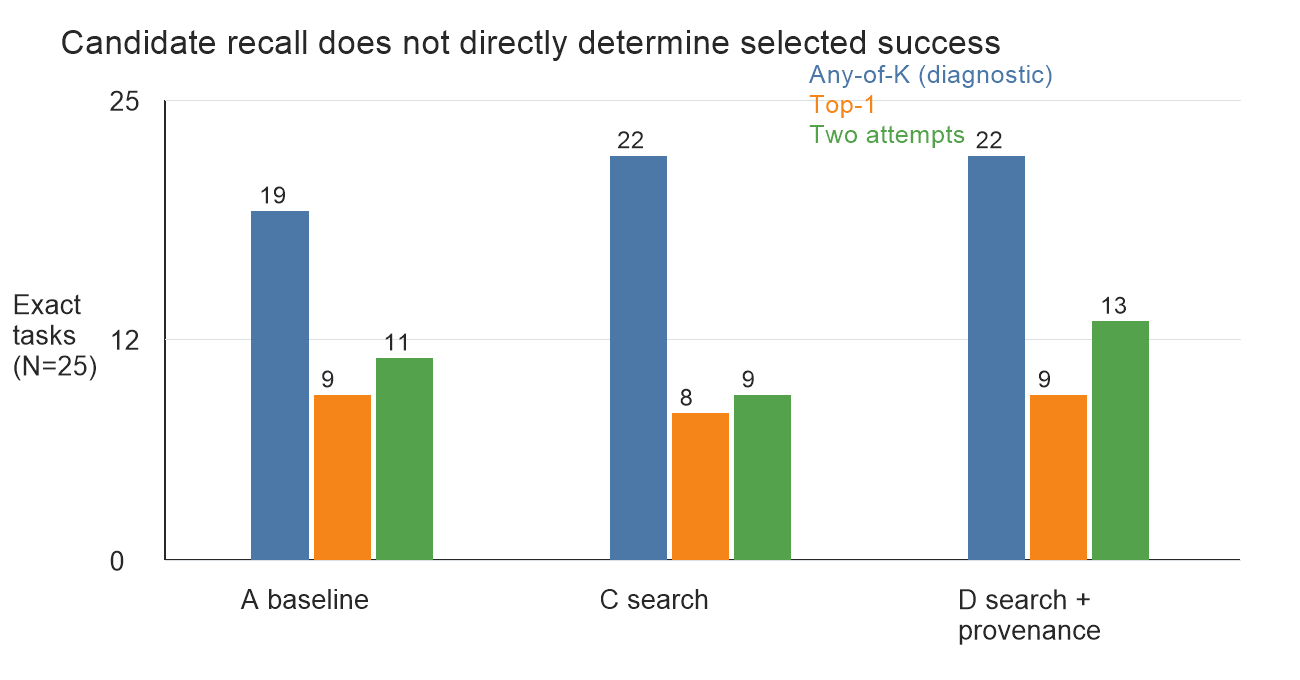
\includegraphics[width=.87\linewidth]{figures/frozen30_recall_selection.png}
\caption{Partial frozen30 diagnostic (N=25 complete tasks). Search changed recall more than Top-1; provenance-aware selection changed the two-attempt portfolio.}
\label{fig:frozen30}
\end{figure}

\section{Experimental protocol}
The stronger studies precommit or hash task selection and configuration before inference. Candidate pools and selected ranks are frozen before solutions can be opened by a separate scoring phase. The untouched60 manifest records 60 task IDs selected from a held-out source split, explicit exclusions of historical exposure, immutable method hashes, and no target inspection. This protocol does not eliminate every possible cohort effect, but it prevents post-score selector changes within the documented study.

The freeze boundary is operational rather than rhetorical. Before a scored condition, the repository records the cohort-selection procedure, model/interface identity, decoding budget, augmentation definitions, seed or deterministic policy, selection rule, and solution-access constraint. Generation consumes task training pairs and test inputs, but no test targets. In the symbolic path, a candidate is executed against all available training pairs and retained only if it passes the deterministic hard verifier. In the native path, exact candidate grids are grouped across all test inputs for a task; the group retains its generation provenance when the artifact format permits it. The ranker then orders groups using the predeclared train-only likelihood or support rule. A two-attempt submission is the first and next distinct output in that frozen order, not a post-hoc pair chosen after seeing a target.

This distinction matters for interpreting comparisons. The untouched60 A/B study holds candidate generation fixed: B is a selection change over a frozen A pool, not a claim that B generated more correct grids. In contrast, the frozen30 A/C comparison changes the candidate pool through a fixed 32-view, four-branch search budget, while C/D holds that new pool fixed and changes selection. The partial frozen30 report admits only tasks with an atomic checkpoint containing all 32 augmentations and 128 raw generations, a valid candidate pool, and a matching checkpoint identity. Five incomplete tasks were excluded before the scored subset was formed. These safeguards do not make diagnostic cohorts representative of competition evaluation, but they make the interpretation of each local contrast explicit.

The reported metrics answer different questions. Any-of-K becomes observable only after scoring and should be read as candidate-pool recall, not an inference-time solver rate. Top-1 measures the first ranked output and tests selector quality under a one-answer policy. Two-attempt exact success measures the portfolio induced by the fixed first two distinct ranks. In the paired untouched60 comparison, B solved four tasks that A did not and A solved one that B did not. The exact two-sided binomial p-value over those five discordant pairs is 0.375; this small paired sample supports neither a statistical-significance claim nor a conclusion that the observed difference will persist on another cohort.

\section{Results}
Table~\ref{tab:results} is a cohort-preserving summary. It should not be read as one leaderboard.

\begin{table}[t]
\centering\small
\begin{tabular}{p{.23\linewidth}r p{.27\linewidth} p{.34\linewidth}}
\toprule
Cohort & N & Method / metric & Result and qualification\\
\midrule
V2 frozen pilot & 50+50 & Macro DSL exact & 0/50 in symbolic and direct routes; retained negative result\\
V3 construction audit & 30 & exact train coverage & 3/30 $\rightarrow$ 10/30; train-only representability\\
frozen30 forensics & 30 & Any-of-K / Top-1 & 21/30 / 9/30; diagnostic rank analysis\\
partial frozen30 & 25 & D recall / Top-1 / two attempts & 22/25 / 9/25 / 13/25; incomplete five excluded\\
untouched60 A/B & 60 & two-attempt exact & 18/60 vs 21/60; paired $p=0.375$\\
scheduler replay & 60 & modeled makespan & 7,557.76 s $\rightarrow$ 5,564.09 s; CPU-only replay\\
\bottomrule
\end{tabular}
\caption{Canonical results. Metrics stay with their own cohorts and validation scopes.}
\label{tab:results}
\end{table}

On untouched60, both A and B had diagnostic Any-of-K recall of 30/60. A's Top-1 and two-attempt values were both 18/60; B's were 16/60 and 21/60. There were four B-only and one A-only two-attempt solves among five discordant pairs, giving a recorded exact two-sided binomial $p=0.375$. The Wilson intervals for the two-attempt proportions overlap. The result is therefore reported as an achieved directional difference, not as statistically significant improvement.

\begin{figure}[t]
\centering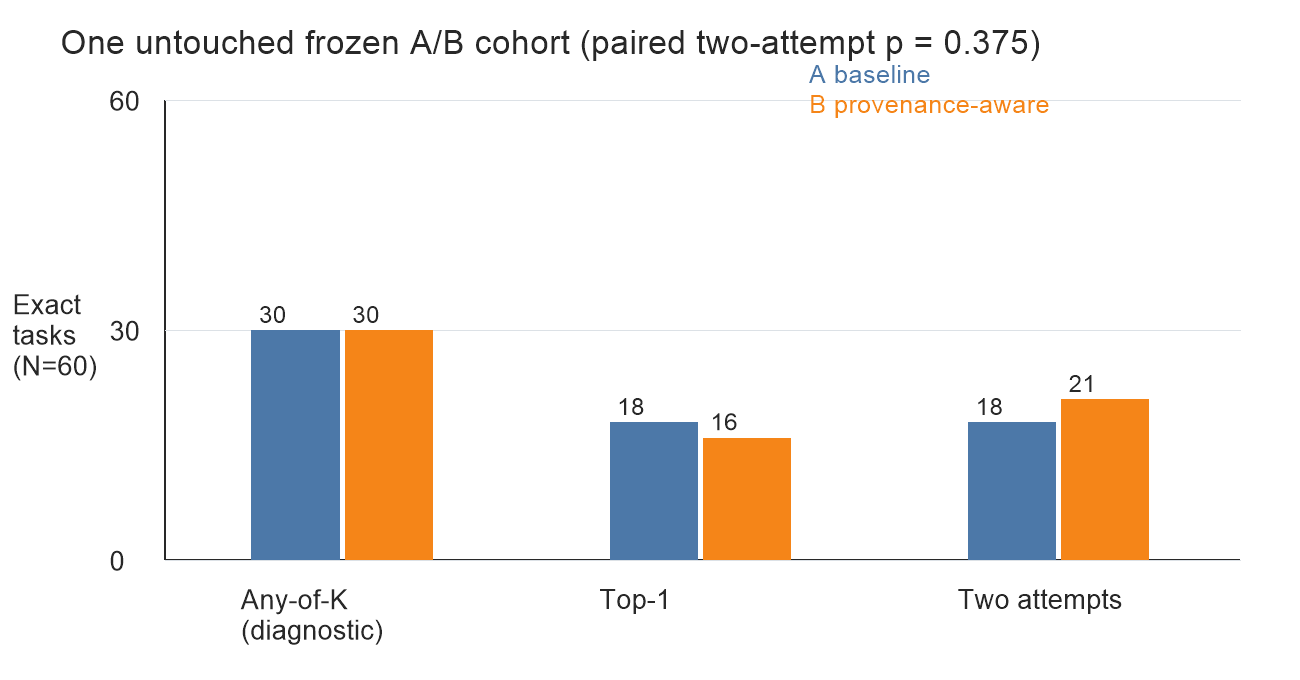
\includegraphics[width=.82\linewidth]{figures/untouched60_ab.png}
\caption{One untouched frozen A/B study (N=60). Any-of-K is diagnostic; two-attempt selection was fixed before target scoring.}
\label{fig:untouched}
\end{figure}

\section{Failure analysis}
The project retains failures as evidence. At the program-synthesis level, syntactic correctness did not guarantee a semantically grounded transformation. At the symbolic level, RuleSpec coverage remains limited by compositional state updates and repeat semantics. At the native inference level, many tasks have no exact candidate at all, while some contain correct candidates ranked below the first output. The partial A/B/C/D study illustrates the consequence: larger candidate pools may improve oracle recall but not Top-1 selection. These are hypotheses for future controlled studies, not claims that one mechanism alone caused each difference.

The records support a more granular taxonomy. A \emph{representation failure} occurs when the available symbolic vocabulary cannot express the train-consistent mechanism; the remaining V3 audit categories include repeat motifs, composition/state update, progressive spacing, and conditional output construction. A \emph{recognition or grounding failure} occurs when a neural planner produces a compile-valid form that does not encode the intended relation. The Macro API sequence illustrates this: compiler-aware constraints reached 60/60 compile validity on an API-only fixed benchmark, while the later deterministic semantic-intent audit recorded semantic grounding failure on 29/60 cases. This is evidence that syntactic interface repair and rule recognition are separate bottlenecks, not evidence that a general ARC recognizer has been solved.

A \emph{generation failure} occurs when no exact candidate is present in a frozen pool after scoring; a \emph{selection failure} occurs when an exact candidate exists but is not first in the fixed ranking. The frozen30 forensics quantify both categories on the same diagnostic set: 9 of 30 tasks had no correct candidate under the recorded pool, while 12 further tasks had a correct candidate but not a Top-1 likelihood selection. The correct-candidate rank distribution is heterogeneous (median two, with some ranks substantially lower), which cautions against treating raw model likelihood as a calibrated correctness estimate. The next research step is therefore not simply a larger candidate budget: it is a preregistered study of target-blind evidence that can distinguish plausible but incorrect candidates from correct ones.

\section{Systems engineering for multi-GPU inference}
The production implementation supports complete model replicas per L4, atomic task checkpoints, resume/no-duplicate semantics, and a dynamic shared task queue. A four-L4 runtime audit records four NVIDIA L4 devices with 23,034 MiB each. The dynamic scheduling result is intentionally conservative: it replays frozen per-task elapsed times on CPU. Static round-robin allocation has a modeled 7,557.76-second makespan versus 5,564.09 seconds for dynamic allocation, a 26.38\% reduction, and estimated utilization changes from 72.81\% to 98.90\%. This shows that task assignment can affect observed throughput without changing candidate-generation semantics; it is not a fresh live-GPU performance claim.

\begin{figure}[t]
\centering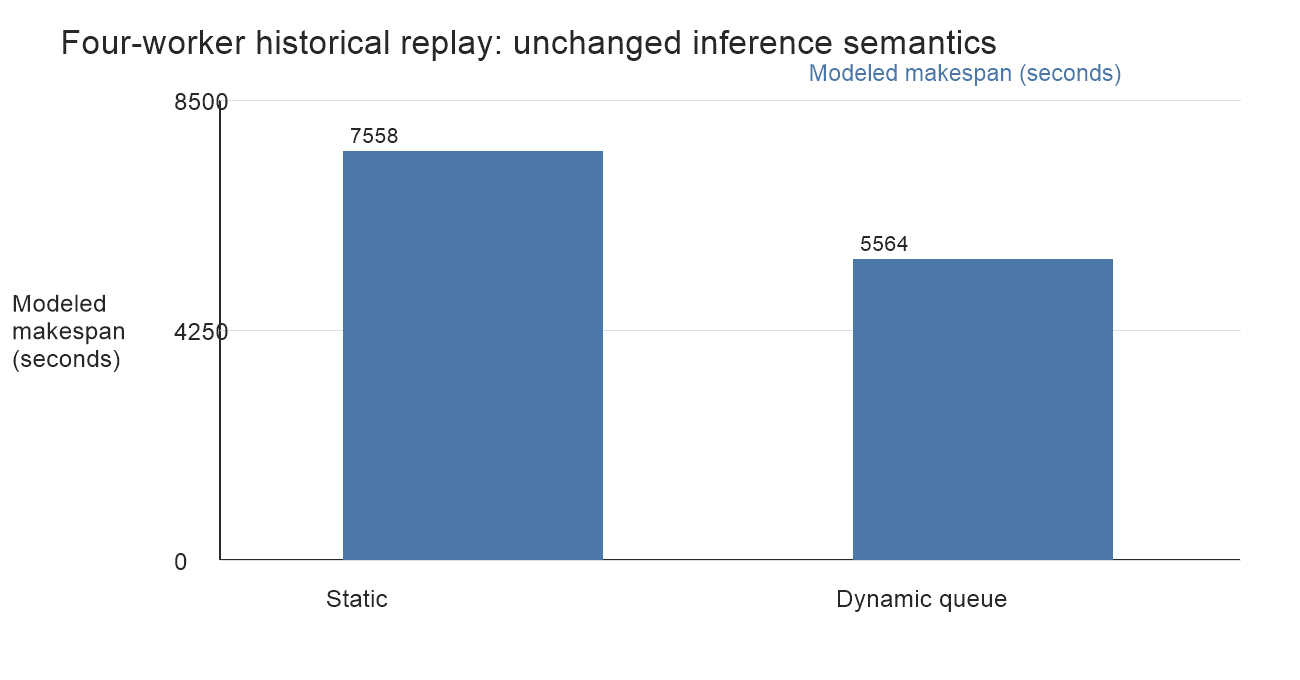
\includegraphics[width=.72\linewidth]{figures/scheduler_replay.png}
\caption{Historical 60-task runtime replay. The values are deterministic modeled makespans, not new GPU measurements.}
\label{fig:scheduler}
\end{figure}

\section{Limitations}
The cohorts are small and heterogeneous. The strongest held-out A/B result has limited power and is not statistically significant. Public pretrained model dependence restricts reproducibility and interpretation. Candidate recall is target-dependent post-hoc diagnostics and cannot be used at deployment. RuleSpec construction evidence is train-only. Some detailed artifacts are private or ignored because they may contain restricted competition data or generated predictions; public claims cite their scope and retain contemporaneous versioned reports where possible. Finally, internal diagnostic cohorts are not the competition hidden test set.

\section{Discussion and conclusion}
This project reframes ARC inference as a chain of inspectable decisions. Deterministic execution and hard verification constrain symbolic hypotheses; frozen protocols constrain evaluation; provenance-aware candidate portfolios expose selection as an explicit object of study; and systems engineering makes expensive inference resumable. The evidence does not support a claim of an effective general ARC solver, a public leaderboard score, a rank, or a medal. It does support a research agenda: improve target-blind candidate-quality estimation, test it on preregistered larger cohorts, and extend compositional symbolic semantics while preserving auditability.

\appendix
\section{Protocol details}
Frozen studies separate inference from scoring. The untouched60 A/B artifacts record the task list, method and configuration hashes, pre-inference freeze, post-prediction scoring gate, and paired outcome sets. Partial frozen30 reports list all included and excluded task IDs. Candidate generation uses fixed augmentation/search budgets, exact output deduplication, and predeclared distinct attempts.

\section{Reproducibility}
The public repository supports Python 3.11+ CPU tests and configuration inspection. GPU replay requires separately acquired ARC data, external public model assets, appropriate PyTorch/CUDA tooling, and historically four L4 GPUs for matching production topology. No raw datasets, test solutions, checkpoints, raw completions, or credentials are distributed. See \texttt{REPRODUCIBILITY.md} and \texttt{docs/EXPERIMENT\_INDEX.md}. Code and public documentation are available in the linked repository; restricted competition artifacts, private predictions, and externally licensed model assets are not redistributed.

{\footnotesize
\bibliographystyle{plain}
\bibliography{references}
}
\end{document}
